\chapter{Implementation of the transformation}
\label{chap:implementation}
%===============================%
%         Trafo stages          %
%===============================%
In this chapter, some details of the transformation implementation will be presented. As mentioned before in section \ref{sec:vsdt}, the transformation process in the VSDT is divided into 5 stages. We've also mentioned that the default validation and structure mapping provided by the transformation framework are reuseable. For the implementation of the new transformation, the framework's DefaultBpmnValidator and BPMN2StrucBPMNTransformation are being reused, as we can see in Figure \ref{fig:implementation_stages}.

\begin{figure}[h]
	\centering		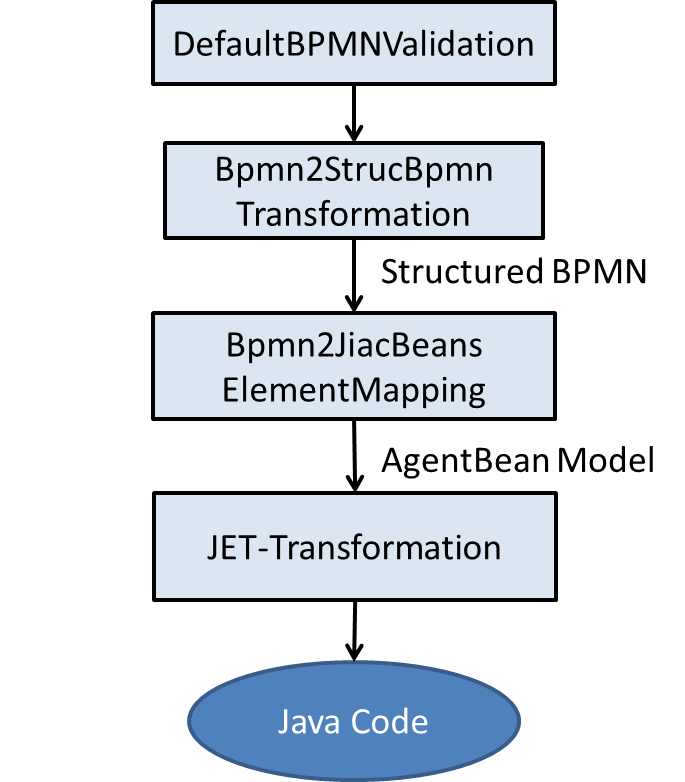
\includegraphics[width=0.5\textwidth]{images/implementation_stages.png}
	\caption{Transformation stages}
	\label{fig:implementation_stages}
\end{figure}

Let's take a look at the details of the newly implemented Stages: Bpmn2JiacBeansElementMapping and the JET-Transformation.

%===============================%
%       Element Mapping         %
%===============================%
\section{Bpmn2JiacBeansElementMapping}
This stage is implemented with the basis of the existing Bpmn2JiacV- ElementMapping. It takes a structured Bpmn as a model and transforms each pool contained in the model's business process diagram into a java object, which represent a model of a java file holding an AgentBean class.\\ For this implementation, a Metamodel of the Jiac AgentBean(see Figure \ref{fig:agentbean_metamodel}) was developed as an intermediate product. An AgentBean model has a list of attributes, methods, action and may also have some subprocess(because a subprocess is mapped into an innerclass of the generated AgentBean). As a model describing the content of a method, a Script-Model was also developed. A script is basically a java code elements, which can be a single CodeElement(a single line java code), a sequence which contains a list of scripts, or even a block construct such as the while loop, or a try-catch block. 

\begin{figure}[h]
	\centering		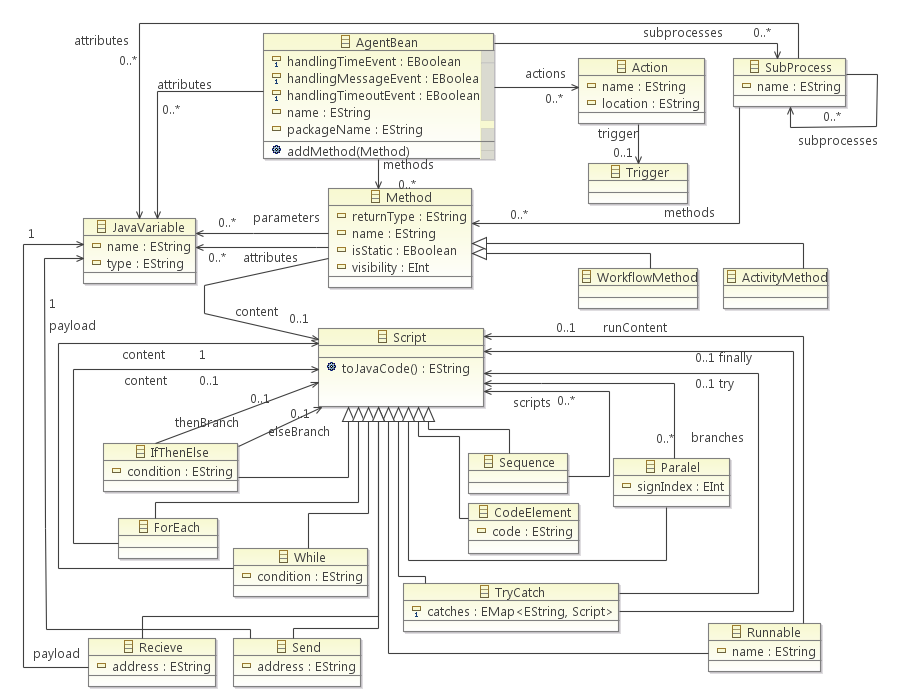
\includegraphics[width=1.0\textwidth]{images/agentBean_metamodel.png}
	\caption{AgentBean - Metamodel}
	\label{fig:agentbean_metamodel}
\end{figure}
